%!TEX root = ../doc.tex
\chapter{Recherche}
\label{sec:recherche}

\section{Kurier-, Express- und Paketdienstbranche}
\subsection{Schweiz}
Die Kurier-, Express- und Paketdienstbranche (kurz KEP-Branche) ist ein altes und unscheinbares Gewerbe. In der Schweiz konnte sich der KEP-Markt erst ab 1997 entwickeln, weil zuvor die schweizerische Post (Post AG) ein Monopol auf den gesamten Inland-KEP-Markt hatte. Das Postgesetz vom 30. April 1997 \citep[]{postgesetz.sr783} öffnete diesen Markt für private Anbieter. Ab dem ersten 1. Januar 1998 war es per Gesetz für private KEP-Anbieter erlaubt, Pakete mit einem Gewicht über 2 Kg und alle Expresssendungen zu transportieren. Am 1. Januar 2004 wurde das Gewichtslimit für Pakete auf 1 Kg gesenkt und per 1. April 2009 auf 50 Gramm womit die schweizerische Post nur noch ein Teilmonopol auf den inländischen Briefmarkt hat. Seit der Öffnung des KEP-Marktes haben sich in der Schweiz einige private KEP-Dienstleistungsanbieter etabliert und unter dem Dachverband KEP\&Mail\footnote{Siehe Abbildung \ref{fig1:kepmail}} organisiert.
\begin{figure}[ht]
	\centering
  
\includegraphics[width=0.66\textwidth]{images/kepmailMitglieder.png}
	\caption{Mitglieder von KEP\&Mail}
	\label{fig1:kepmail}
\end{figure}
Der Dachverband publiziert keine Zahlen bezüglich Marktanteilen der einzelnen Mitglieder. Im Jahresbericht 2015 \citep[S.32]{postCom.2015} der PostCom, einer unabhängigen Regulierungsbehörde des schweizerischen Postmarktes, welche durch das neue Postgesetz im Oktober 2012 ins Leben gerufen wurde, werden aber Zahlen zum gesamten KEP-Markt publiziert. Der KEP-Markt (Pakete bis 30Kg, National, Import, Export) mit einem Volumen von 150 Millionen Paketen wird zu 25\% von Kurier- und Expressdienstleistern bestritten. Beim Import und Export von Paketen wird ca. 80\% des Volumens von privaten Anbietern abgearbeitet. Beim inländischen Versand von Paketen kommen die privaten Anbieter nur auf 20\% Umsatzanteil\footnote{Siehe Abbildung \ref{fig1:umsatzanteil} Quelle: PostCom Jahresbericht 2015}.
\begin{figure}[ht]
	\centering
  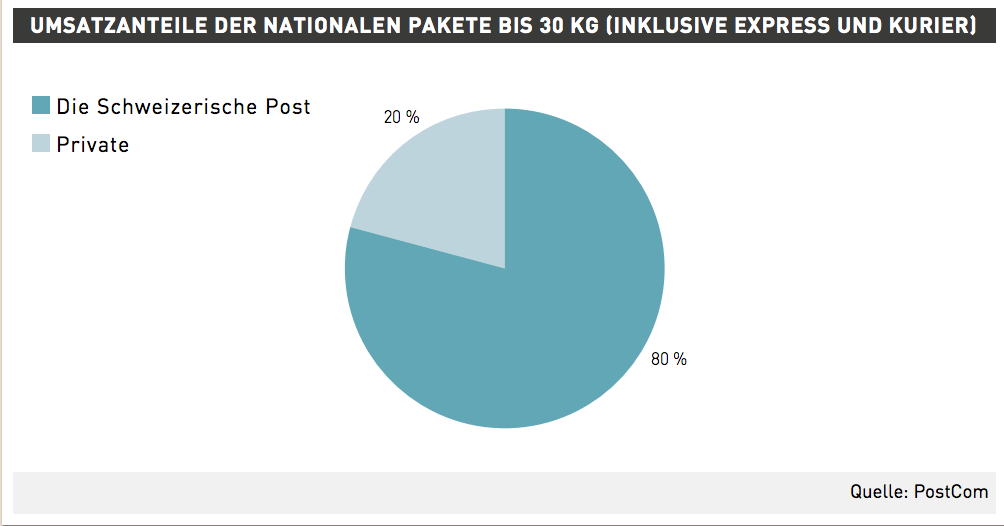
\includegraphics[width=0.88\textwidth]{images/umsatzanteilNational.png}
	\caption{Umsatzanteil der Nationalen Pakete} %Quelle: postCom Jahresbericht 2015
	\label{fig1:umsatzanteil}
\end{figure}
Der Jahresbericht zählt die Post, DPD und DHL Express zu den grössten Anbieter von Paketdienstleistungen in der Schweiz. FedEx, UPS, GO und TNT sind die grösseren internationalen Mitanbieter von Paketdienstleitungen in der Schweiz.

\subsection{Europa}
Informationen und Zahlen zum KEP-Markt in Europa sind rar und schwierig zu finden. Im Jahre 1999 haben sich sieben KEP-Dienstleistungsanbieter (DHL, DPD, General Parcel Austria, Österreichische Post,
TNT, trans-o-flex und UPS) zu einem sogenannten KEP-Forum zusammen geschlossen, jedoch bereits 2005 wieder aufgelöst wurde, weil 2004 interne Preisabsprache vermutet wurde und die gemeinsame Plattform sich nicht in die Richtung entwickelt habe, wie ursprünglich angenommen \citep[S. 14]{mencler2006KEP}. Allerdings ist anzunehmen, dass sich KEP-Märkte in Mitteleuropa gleichen. Der grösste KEP-Markt in Europa ist in Deutschland zu finden. 2011 machte dieser  36.9\% aus\footnote{Siehe Abbildung \ref{fig1:marktanteil} Quelle: WIK-Consult, Main Developments in the Postal Sector (2010-2013), Study for the European Commission, DG Internal Market and Services}.
\begin{figure}[ht]
	\centering
  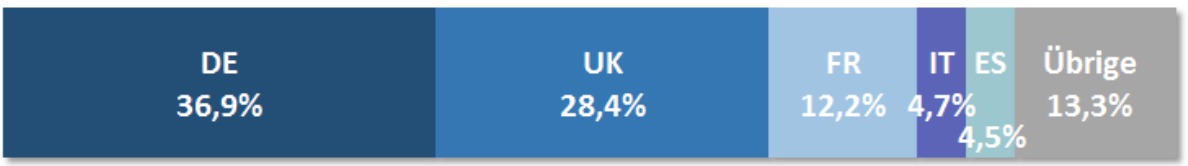
\includegraphics[width=0.88\textwidth]{images/kepMarktEuropa2011.png}
	\caption{Europäischer Kurier-, Express- und Paketmarkt im Jahre 2011} %Quelle: postCom Jahresbericht 2015
	\label{fig1:marktanteil}
\end{figure}
Europäische KEP-Märkte weisen oligopolistische Tendenzen auf, weil ein Grossteil des Umsatzes von einigen wenigen Anbietern erzielt wird (DHL, DPD, FedEx, TNT, UPS)\citep[S.14]{baum2004produktivitats}. Jedoch bieten diese Marktstrukturen ein grosses Potenzial für innovative Unternehmen, welche nicht mit der Philosophie der zuvor genannten Anbietern arbeiten.


\section{Standards und Software}
Obwohl es gewisse Standards für die Kurier-, Express- und Paketdienstbranche gibt, sind die meisten System, welche bei den Anbietern im Einsatz sind eigene Entwicklungen. Diese Entwicklungen sind proprietär und bieten meistens ihre eigenen Benutzeroberflächen beziehungsweise Weboberflächen für Endkunden an. Grössere Anbieter stellen Schnittstellen zu ihren Systemen zur Verfügung, folgen dabei jedoch keinem Standard. So brauchen Module wie z.B XSI (eXpress Shipper Interface) als Teil von SAP\footnote{SAP ist ein ERP-System}, welche auf einen elektronischen Datenaustausch vorbereitet sind, immer noch zusätzliche Komponenten, welche zwischen den Systemen übersetzten.
\newline{}
Standards, welche seit langer Zeit in der Branche genutzt werden, sind EDIFACT beziehungsweise EDITRANS, welche zu Zeiten ihrer Einführung über Telex System kommunizierten. Mit dem Aufkommen von Fax und Email verloren Telex Systeme und auch teilweise die Standards an Bedeutung. Telex und die Standards sind aber immer noch bei den ganz grossen KEP-Anbietern, welche eine eigene Flugzeugflotte betreiben, (z.B. Fedex) zu finden.

\subsection{EDIFACT}
UN/EDIFACT steht für \textit{United Nations Electronic Data Interchange For Administration, Commerce and Transport} und ist Teil der internationalen EDI-Standards. EDI (Electronic Data Interchange)-Standards wurden für den elektronischen Datenaustausch zwischen Unternehmen oder durch Normierungsvorschläge von Branchenverbänden entwickelt. Unter den EDI-Standards findet sich auch SWIFT, welcher für den Datenaustausch zwischen Banken genutzt wird. Das UN zu Beginn des offiziellen Namen des Standards steht für \textit{United Nations} (Vereinte Nationen), welche mit der Einrichtung CEFACT (\textit{Centre for Trade Facilitation and E-Business}) für den Standard verantwortlich ist. Aufgrund der Grösse und Komplexität von EDIFACT wurden für die verschieden Branchen sogenannte \textit{Subsets} erstellt. Im Folgenden eine nicht vollständige Liste mit Namen und Zugehörigkeit verschiedener Subsets \citep[S.1]{thopasEDIFACT}.
\begin{description}
	\item [EANCOM] Konsumgüterindustrie
	\item [EDIFOR] Speditionsbranche
	\item [EDIFURN] Möbelbranche
	\item [EDILIBE] Buchhandel
	\item [EDITRANS] Transportwirtschaft
	\item [EDIWHEEL] Reifen- und Räderhersteller
\end{description}
Im EDIFACT Standard sind ca. 200 verschiedene Nachrichtentypen für die unterschiedlichsten Anwendungszwecke definiert. Jede Nachricht wird durch einen sechsstelligen Namen eindeutig gekennzeichnet. Im Folgenden eine nicht vollständige List mit einigen Beispielen.
\begin{description}
	\item [IFTMBF] Buchungsanfrage (transport booking request)
	\item [IFTMBC] Buchungsbestätigung (transport booking confirmation)
	\item [IFTMIN] Transport-/Speditionsauftrag (instructions of transport)
	\item [ORDERS] Bestellung (purchase order message)
	\item [PRICAT] Preisliste/Katalog (price catalogue message)
\end{description}
Im Folgenden ist eine EDIFACT Nachricht, welche auf eine Verfügbarkeitsanfrage für einen Flug zwischen Frankfurt und Miami zurückkommt.
\begin{verbatim}
UNA:+.? '
UNB+IATB:1+6XPPC+LHPPC+940101:0950+1'
UNH+1+PAORES:93:1:IA'
MSG+1:45'
IFT+3+XYZCOMPANY AVAILABILITY'
ERC+A7V:1:AMD'
IFT+3+NO MORE FLIGHTS'
ODI'
TVL+240493:1000::1220+FRA+JFK+DL+400+C'
PDI++C:3+Y::3+F::1'
APD+74C:0:::6++++++6X'
TVL+240493:1740::2030+JFK+MIA+DL+081+C'
PDI++C:4'
APD+EM2:0:1630::6+++++++DA'
UNT+13+1'
UNZ+1+1'
\end{verbatim}
Die erste Zeile mit \textit{UNA} wird in allen EDIFACT-Nachrichten benötigt. Sie definiert die Trennzeichen der Nachricht fest. Darauf folgt mit \textit{UNB} ein \textit{Interchange Header} und danach mit \textit{UNH} die eigentliche Nachricht, welche bei \textit{UNT} wieder endet. Mit \textit{UNZ} endet die Nachricht.
\newline{}
Obwohl der EDIFACT Standard viele Geschäftsprozesse abdecken könnte, wird er nur von den grössten Anbietern der Branche eingesetzt. Ein finanzieller Gewinn durch den Standard entsteht erst ab einem gewissen Transportvolumen.

\section{LoBo}
Lobo ist eine SaaS Applikation, welche auf die Bedürfnisse von Kurier-, Express- und Paketdienstleistern zugeschnitten ist. Der Service wurde zu Beginn hauptsächlich von Fahrradkurieren eingesetzt, aber wird vermehrt auch von anderen Dienstleistern eingesetzt. Lobo wurde in PHP entwickelt, wird von einem Apache Server ausgeliefert und speichert die Daten in einer Datenbank. Zusätzlich bietet LoBo eine REST (\textit{Representational State Transfer}) API (Application Programming Interface) an, welche mit einem Schlüssel und einer Client Identifikation genutzt werden kann. Die Abbildungen \ref{fig1:lobooverview} und \ref{fig1:lobonewtask} geben einen visuellen Überblick über die Benutzeroberfläche von LoBo.
\begin{figure}[ht]
	\centering
  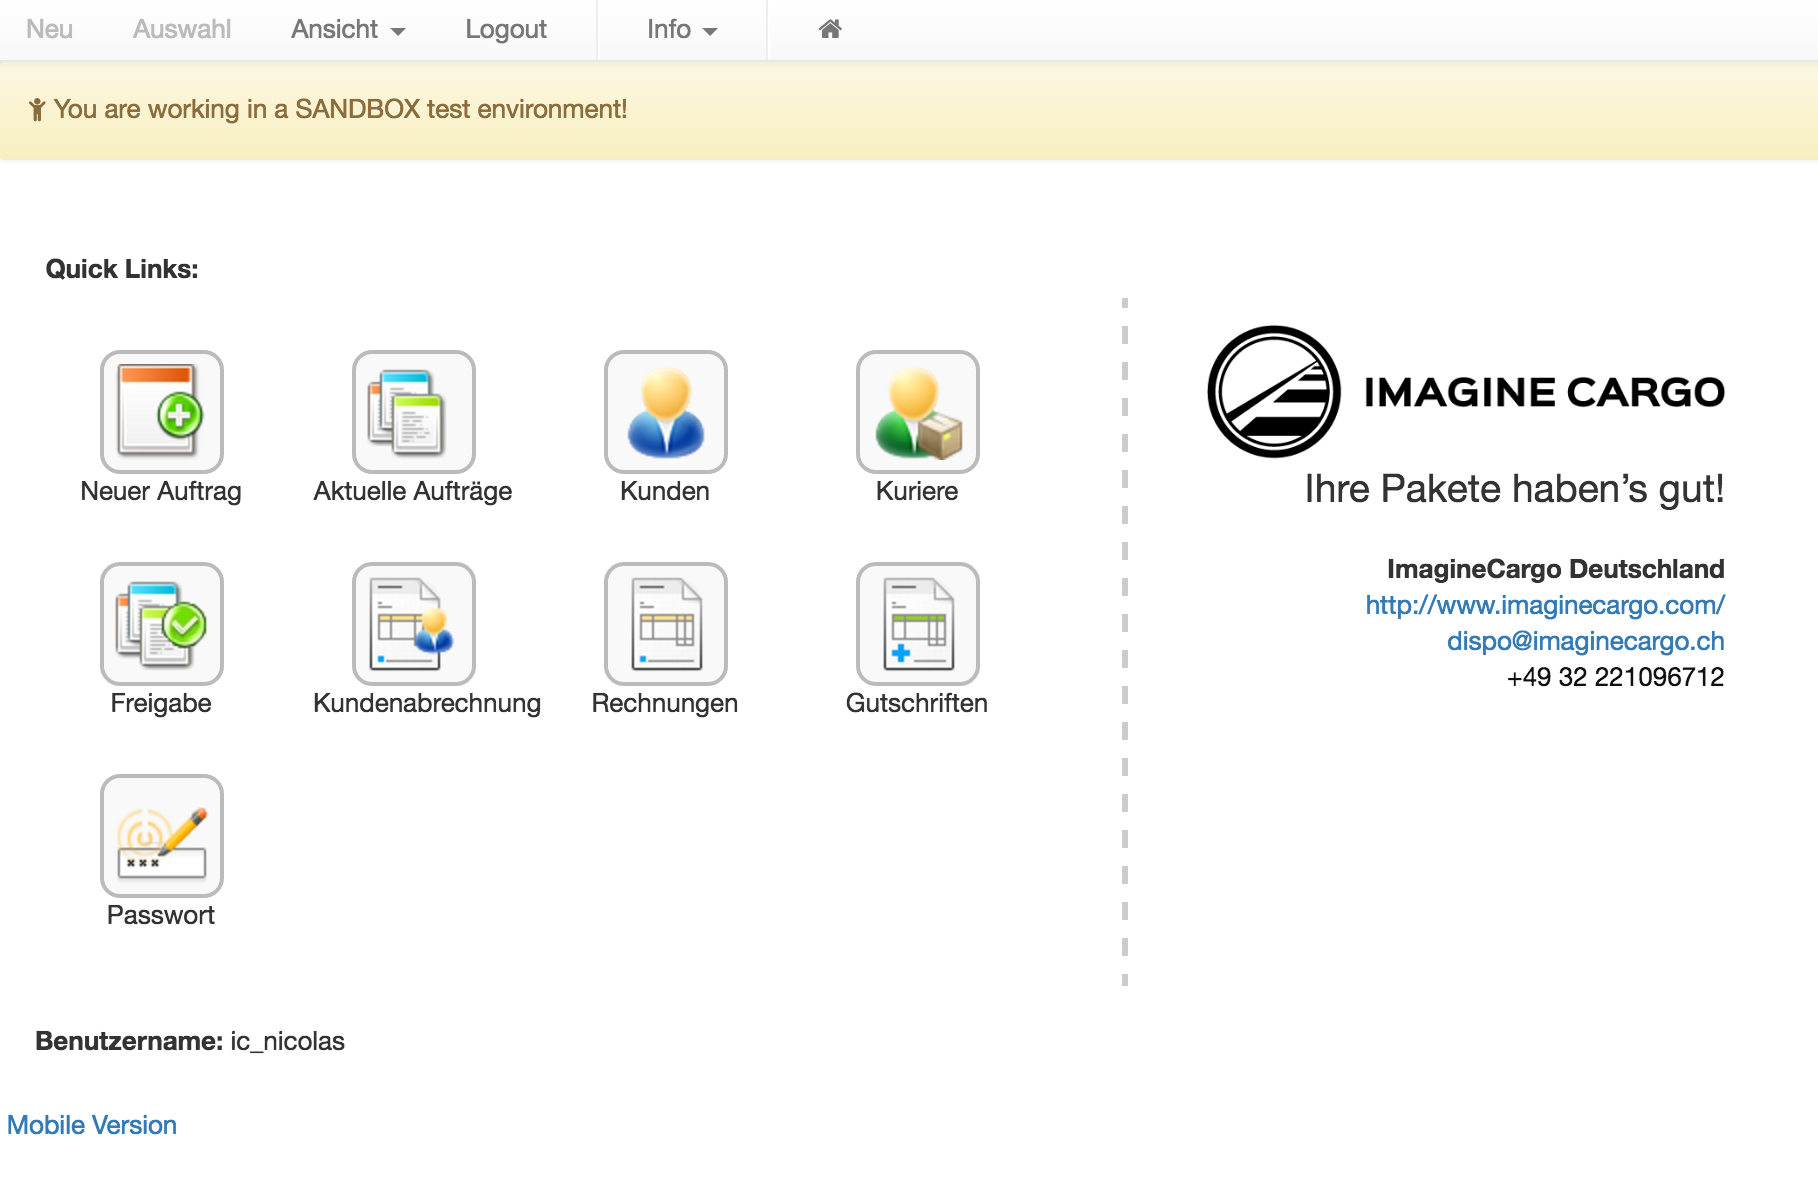
\includegraphics[width=0.88\textwidth]{images/loboOverview.png}
	\caption{Einstiegsmaske von Lobo}
	\label{fig1:lobooverview}
\end{figure}
\begin{figure}[ht]
	\centering
  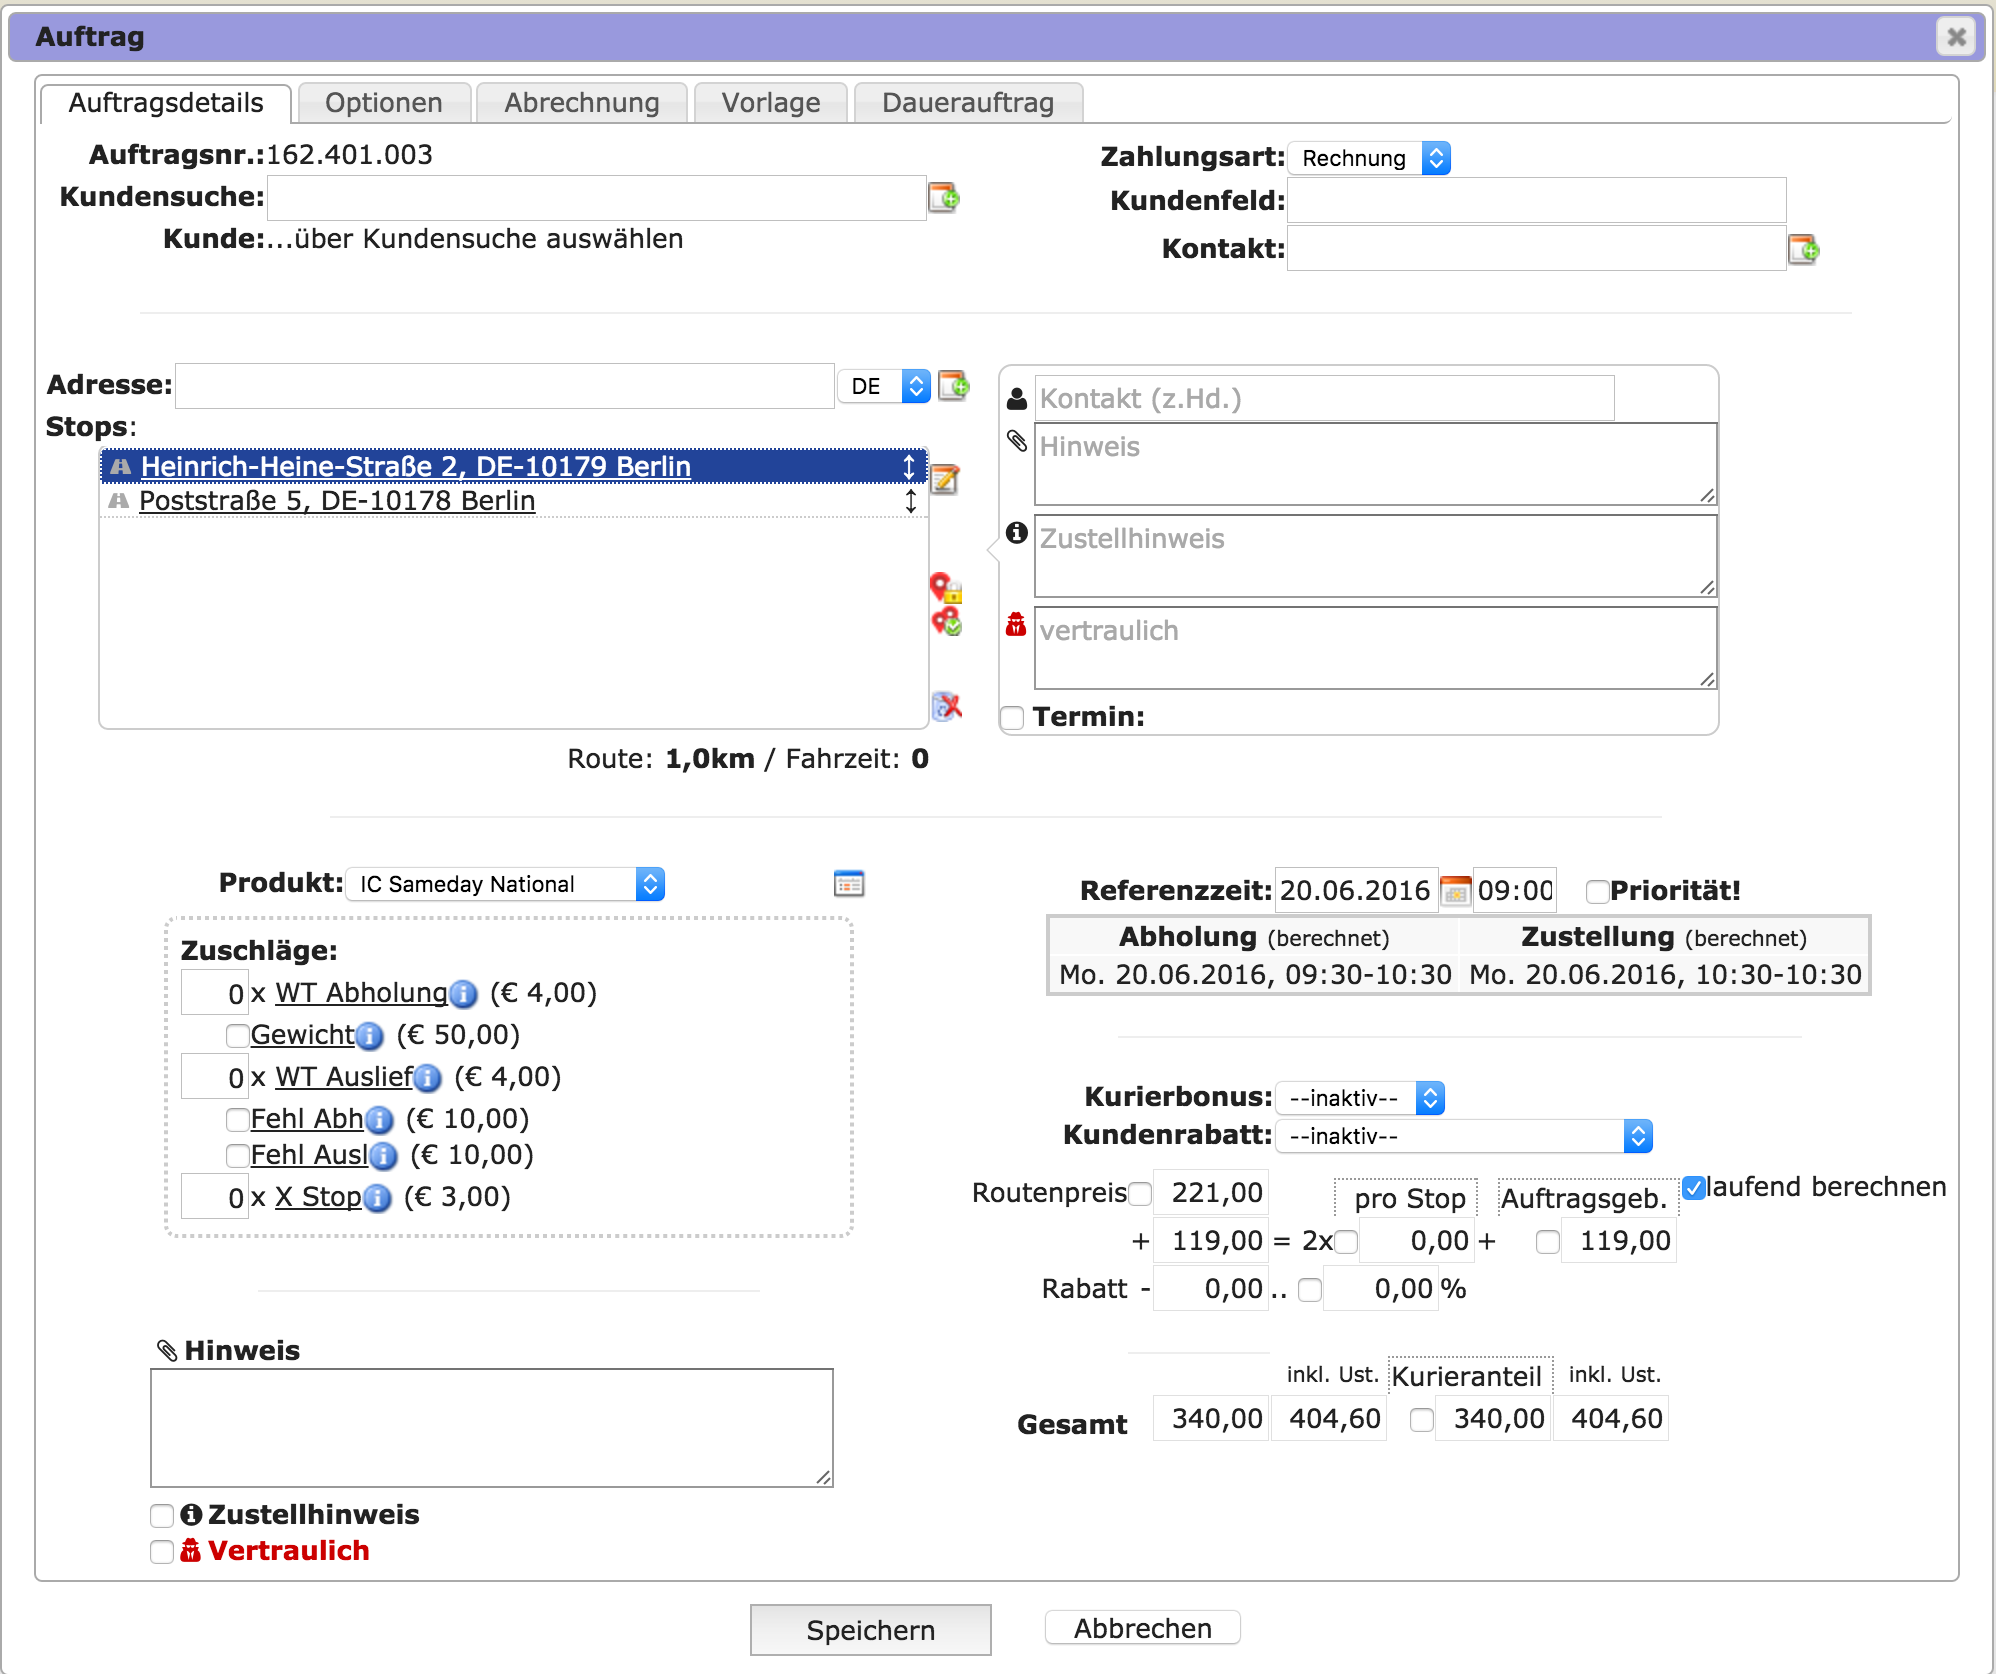
\includegraphics[width=0.88\textwidth]{images/loboNewtask.png}
	\caption{Neuen Auftrag erstellen in Lobo}
	\label{fig1:lobonewtask}
\end{figure}
In Lobo können Zeitmodelle erstellt werden, welche definieren, wie eine Zustellung von Start bis Ende zeitlich abläuft\footnote{Siehe Abbidlung \ref{fig1:lobozeitmodell}}. Diese Zeitmodelle sind die Produkte, welche dem Kunden zur Verfügung stehen.
\begin{figure}[ht]
	\centering
  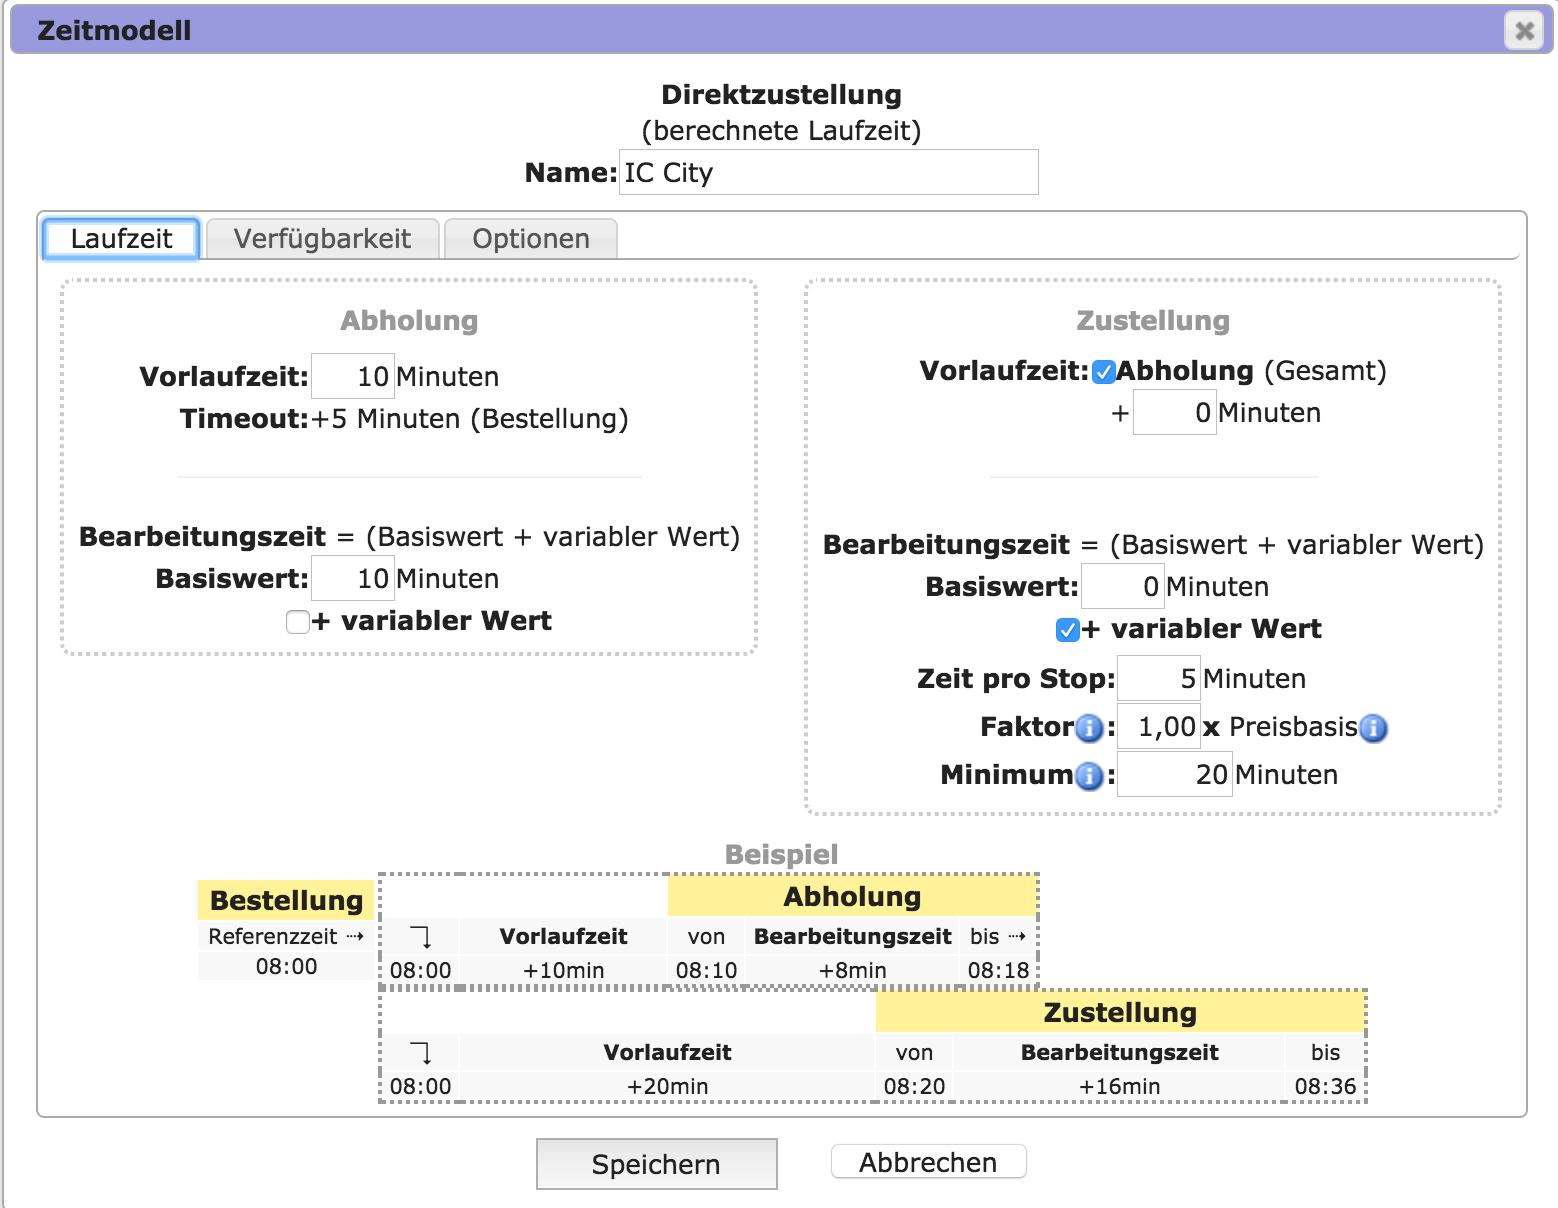
\includegraphics[width=0.88\textwidth]{images/loboZeitmodell.png}
	\caption{Zeitmodell in Lobo}
	\label{fig1:lobozeitmodell}
\end{figure}
Zusätzlich wird eine Preisstaffel erstellt, welche den Preis für die Pakete und Route berechnet\footnote{Siehe Abbildung \ref{fig1:lobopreisstaffel}}.

\begin{figure}[ht]
	\centering
  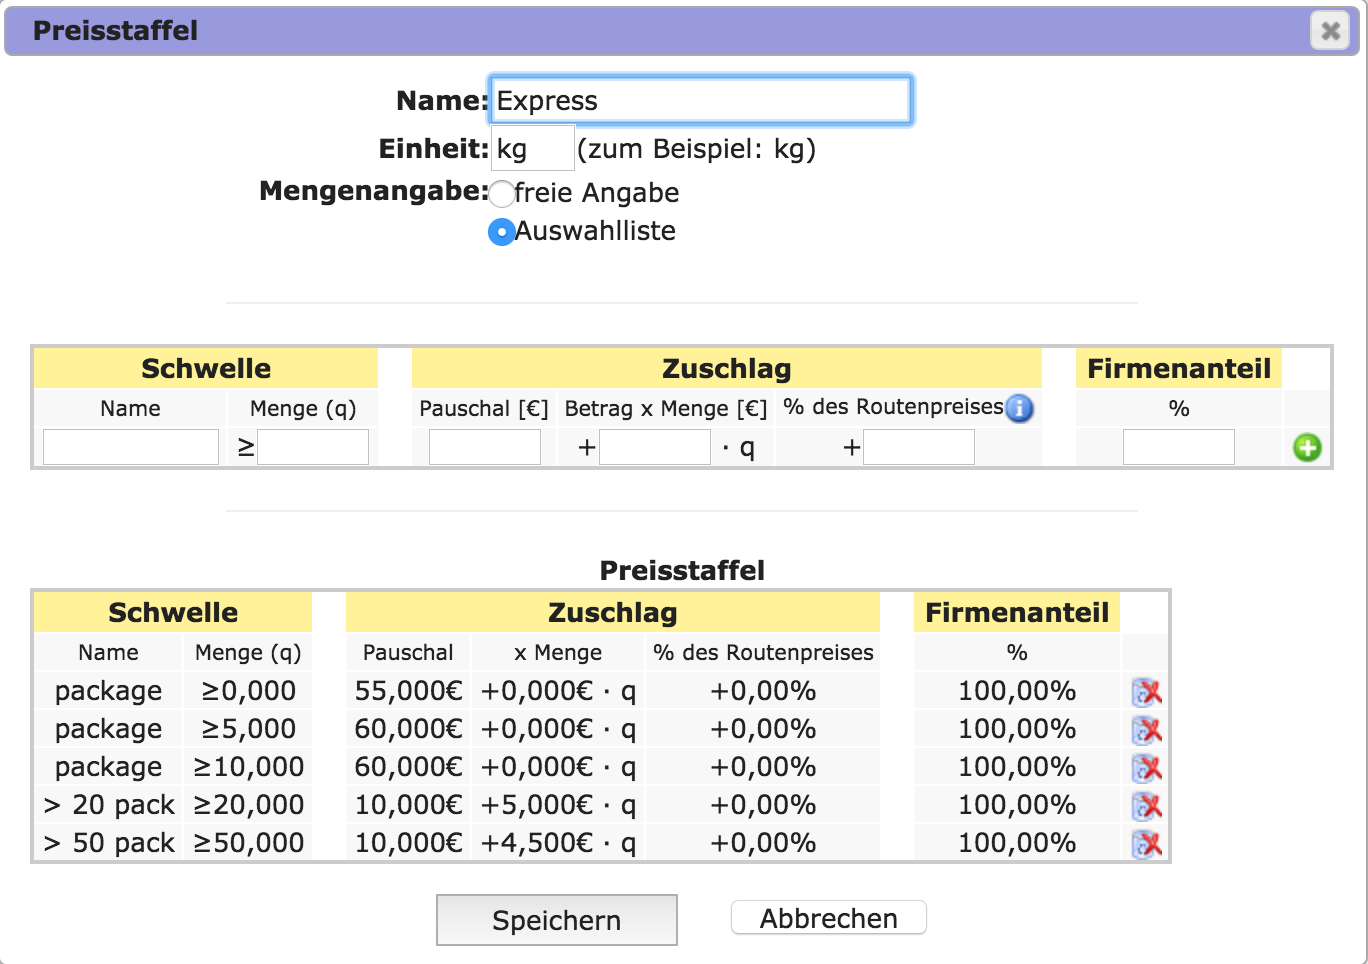
\includegraphics[width=0.88\textwidth]{images/loboPreisstaffel.png}
	\caption{Zeitmodell in Lobo}
	\label{fig1:lobopreisstaffel}
\end{figure}


\subsection{API}

Die API von Lovo kann mit jedem REST-kompatiblen System angesprochen werden. Jede Instanz von LoBo hat einen eigenen API-Endpunkt, welcher über eine URL (Uniform Resource Locator) erreichbar ist. Bei jeder Anfrage werden folgende Parameter zwingend benötigt.
\begin{description}
	\item[action] Die auszuführende Aktion
	\item[clientIp] Die IP-Adresse des Anfragenden
\end{description}
Zusätzlich kann mit \textit{responseFormat} die Enkodierung der Antwort angegeben werden. Standard ist JSON (JavaScript Object Notation). Bei gewissen Aktionen müssen oder können zusätzliche Parameter angegeben werden. Diese Parameter werden als URL-Enkodierte Forms versendet (\textit{application/x-www-form-urlencoded}).
Bevor die Anfrage gesendet werden kann, wird ein Hash über die Parameter berechnet. Die Berechnung findet nach \textit{SHA-256} statt und der API Schlüssel wird dafür verwendet. Der berechnete Hash wird als Hexadezimal im Header der Anfrage mitgeschickt. Zusätzlich wird die Client Identifikation im Header mitgeschickt. Dadurch lässt sich die Authentizität und Integrität der Daten auf dem Server verifizieren. Die API antwortet im gewünschten Format mit numerischen Stati, welche den Erfolg bzw. nicht Erfolg beschreiben und im Falle einer erfolgreichen Anfrage die gewünschten Daten zurückliefert. Im Folgenden eine nicht vollständige Liste mit einigen Beispiel-Anfragen. Die vollständige Liste ist im Anhang \ref{sec:loboAPI} zu finden.

\begin{description}
	\item[getProductList] Benötigt keine Parameter und liefert die oben erwähnten Produkte zurück.
	\item[createTask] Benötigt eine Produkt-Id, eine Bezahlungs-Id und eine Kundennummer. Die Anfrage liefert einen Tasktoken zurück, welcher für die Weiterführung des Auftrags benötigt wird.
	\item[addStop] Benötigt den oben erwähnten Tasktoken, einen dreistelligen Ländercode, eine Postleitzahl, eine Strasse und eine Hausnummer. Die Anfrage liefert die eingeben Daten zurück und eine eindeutige Id.
	\item[calculateTask] Benötigt den oben erwähnten Tasktoken. Liefert bei erfolgreicher Verarbeitung alle Informationen, Zeiten und Kosten des Auftrages zurück.
\end{description}
